\chapter{INTRODUCTION}
\section{Background}
\label{section:background}
    \begin{figure} [H]
        \centering
        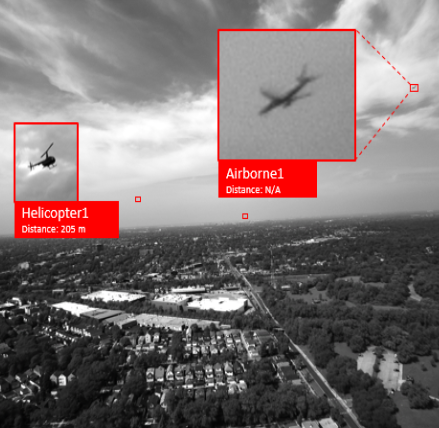
\includegraphics[width=0.5\textwidth]{figures/dataset-example-labeled.png}
        \caption{An example of airborne object dataset}
        \label{fig:airborne-object-example-1}
    \end{figure}
    \vspace{-2ex}
    %Seiring berkembangnya teknologi \emph{autonomous vehicles}, terdapat banyak keinginan untuk mengaplikasikan teknologi tersebut di berbagai bidang.
    %Salah satu aplikasi teknologi ini di bidang komersil adalah \emph{Amazon Prime Air}.
    %\emph{Amazon Prime Air} memanfaatkan \emph{Autonomous Aerial Vehicle} (AAV) untuk melakukan pengantaran barang dari warehouse ke rumah kostumer secara \emph{autonomous} \parencite{prime_air}.
    %Untuk melakukan hal ini, AAV yang digunakan harus mempunyai kemampuan penerbangan \emph{autonomous} yang mumpuni.

    %One of the most critical challenges in designing such a system is the 
    %ability to sense and avoid (SAA) obstacles. Although the airspace in 
    %which AAV operate is relatively sparse, there is still a risk of 
    %encountering static obstacles or airborne objects such as birds or drones.
    %In commercial application, such encounter would result not only in the AAV,
    %but also the item which the AAV carries.
    %Airborne objects pose a particularly difficult challenge as they often appear 
    %unexpectedly and approach rapidly from long distances due to their
    %inherent need for speed in flight.

    Autonomous Aerial Vehicle (AAV) have the potential to significantly impact 
    industries, particularly in commercial delivery. One notable example is Amazon 
    Prime Air, which is currently under development. Prime Air aims to deliver 
    goods from Amazon warehouses directly to customers \parencite{prime_air}. 
    To accomplish this, AAV require a reliable and efficient autonomy system.
 
    One of the most critical challenges in designing an AAV system is the 
    ability to sense and avoid (SAA) obstacles. While the airspace in which 
    AAVs operate may be relatively sparse, there is still risk of encountering 
    static obstacles or airborne objects such as birds or drones. In commercial 
    applications, such encounters can have consequences not only for the AAV 
    itself but also for the items it carries.  Ensuring effective SAA 
    capabilities is essential to mitigate these risks and safeguard both the AAV 
    and the valuable cargo it transports.


    Most SAA system of AAVs includes camera as their primary sensor.
    Cameras provide visual perception to the AAV, real-time, in the form of images. 
    These images must be processed by a computer vision algorithm to identify
    and localize the obstacles in it so that the AAV can estimate their 
    position and plan actions it needs to do to avoid them.
    There are other onboard sensing options such as LiDAR or radar, but cameras
    are more favored due to their lighter weight, cheaper price, 
    and relatively lower energy consumption compared to active sensors. 

    Airborne objects present a particularly challenging problem in SAA as they can 
    appear unexpectedly and approach rapidly from long distances due to their 
    inherent need for speed in flight. For this reason, it is important to detect airborne
    objects while they are still far away. Unfortunately, their far distance cause them 
    to appear very small on images. Figure \ref{fig:airborne-object-example-1} show an
    example of how airborne objects appear on images. In \textcite{aot_docs}, the airborne 
    objects can appear in the range of 4 to 1000 px on a $2048 \times 2448$ px image, that is,
    around 0.00008 - 0.01 \% of the image area.

    For reasons listed above, the computer vision algorithm to be implemented to detect these airborne objects, 
    must be able to detect small objects accurately. And not only that, it also must be able to do it in real-time.
    The fact that AAVs operating environments are outdoors, brings more trouble for the computer
    vision. Outdoor environment brings large complexity and additional variance to the image distribution, 
    making it almost impossible to handcraft feature extractor for it. This is where non-handcrafted
    feature extractors come in handy, particularly the deep learning approaches. Deep learning models
    have shown incredible abilities in handling complex data. Given enough training data, a deep learning
    model can craft itself feature kernels that can extract the objects in an image, despite being subjected
    to complex outdoor environment. For this reason, deep learning models gained prominence in addressing
    these challenges. 
    \begin{figure} [H]
        \centering
        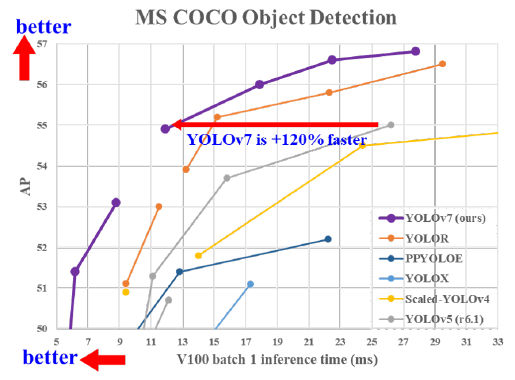
\includegraphics[width=0.5\textwidth]{figures/yolov7-coco.png}
        \caption{YOLOv7 performance on COCO dataset compared to other object detectors.}
        \label{fig:yolov7-coco}
    \end{figure}

    Introducing YOLOv7, a state-of-the-art deep learning based real-time object detector \parencite{yolov7}.
    At the time of the proposal for this research was made (November 2022),
    YOLOv7 outperform both in speed and accuracy of all known real-time object detectors 
    with inference speed in the range of 5-160 FPS. It also has the highest accuracy (56.8\% AP) among
    object detectors with inference speed greater than 30 FPS on a V100 GPU. The capabilities of this cutting-edge architecture
    makes it well-suited for AAV computer vision system. However, all the performance metrics of YOLOv7
    mentioned before are obtained by training the model using COCO 2017 dataset. A dataset which 
    consist of general objects that people see in their daily life. COCO dataset is going to have
    very distinct distribution compared to airborne objects. As such, there would be a need for
    some modification to YOLOv7 so that it could detect airborne objects well.

    The topic of this research is about modifying YOLOv7 with objective of optimizing it to detect
    small objects, which extends to airborne objects. We experimented with some modification to 
    YOLOv7's bag-of-freebies, bag-of-specials, and network architecture. Then we benchmarked the
    modified models against the \textcite{aot_dataset}, and picked the model with the highest AP score
    that can perform inference in real-time.

    %For this to work, the computer vision algorithm must be able to be executed
    %in a real-time scenario, but also must be accurate enough 

    %Introducing YOLOv7. 

    %Dengan memilih kamera sebagai sensor, maka dibutuhkan suatu model computer vision untuk diaplikasikan pada kamera tersebut.
    %Objek - objek \emph{airborne} akan tampak sangat kecil pada kamera seperti yang dapat dilihat pada Gambar \ref{fig:airborne-object-example-1}.
    %Beberapa dataset kamera \emph{airborne} yang memiliki resolusi 20482448 pixel, objeknya dapat berukuran 4 (0.00008\% luas resolusi) hingga 1000 pixel (0.01\% luas resolusi) sehingga terlihat sangat kecil \parencite{aot_dataset}.
    %Oleh karena itu, dibutuhkan suatu model yang dapat mendeteksi objek - objek yang sangat kecil sehingga dapat mendeteksi objek \emph{airborne}.


    %YOLOv7 merupakan model state-of-the-art untuk melakukan pendeteksian objek secara real-time.
    %YOLOv7 memiliki akurasi tertinggi dari semua model pendeteksi objek dengan kecepatan deteksi 30 FPS (yang terpublikasi) pada GPU Nvidia V100.
    %Terdapat versi scaled dari YOLOv7 yang memiliki jumlah parameter yang lebih kecil dan dapat diaplikasikan pada device edge computing \parencite{yolov7}.
    %Oleh karena itu, YOLOv7 ini cocok untuk digunakan pada AAV di mana dibutuhkan suatu pendeteksi objek yang real-time.

\section{Problem Statement}
    
    %YOLOv7 bukan merupakan model deteksi objek umum sehingga YOLOv7 tidak didesain untuk melakukan deteksi objek kecil seperti objek-objek \emph{airborne}.
    %Oleh karena itu, dibuatlah rumusan masalah seperti berikut:
    %\begin{itemize}
    %    \item Apa solusi yang dapat diaplikasikan pada YOLOv7 agar kemampuan deteksi objek \emph{airborne}-nya dapat dioptimalisasi?
    %\end{itemize}
    YOLOv7 is not an object detection model specifically designed to detect small objects or airborne objects.
    Therefore, this research ask the following question.
    \begin{itemize}
        \item What modification can be done to YOLOv7 to improve its abilities in detecting airborne objects?
    \end{itemize}

\section{Purpose}
    The purpose of this research is to find modifications of YOLOv7 that would improve its ability in detecting airborne objects.
    %Adapun tujuan dari tugas akhir ini adalah untuk menemukan solusi untuk mengoptimisasi kemampuan YOLOv7 mendeteksi objek airborne.

\section{Problem Scope}
    % superintelligent AGI
    % solomonoff induction
    In this research, we want to formulate the scope of the problem such that the modifications applied
    on YOLOv7 would not lose its real-time detection ability and is still reasonably computable/trainable.
    Otherwise, we can just run a Solomonoff induction on airborne object data and call the result a modification
    of YOLOv7. Thus, we state the following scopes for the problem.
    \begin{itemize}[noitemsep,topsep=0pt]
        \item YOLOv7 is used as the baseline for modifications. 
        \item The result of modification must be able to perform inference in real-time.
        \item The modified YOLOv7 must be trainable within a reasonable duration using the computational resource
        available, which is a computer which uses consumer GPU Nvidia RTX 2080 Ti.
    \end{itemize}
    %Optimisasi kemampuan deteksi objek kecil hanya akan dilakukan dengan memodifikasi YOLOv7.
    %Modifikasi yang diaplikasikan tidak boleh menyebabkan YOLOv7 untuk tidak dapat melakukan pendeteksian secara \emph{real time}.
    %Target pengaplikasian model ini adalah untuk AAV dengan \emph{computational resource} yang terbatas sehingga model hasil modifikasi harus cukup ringan untuk hal tersebut.
    %%Modifikasi yang mengubah arsitektur YOLOv7 secara signifikan sehingga tidak dapat melakukan pendeteksian secara \emph{real-time} tidak akan diaplikasian.